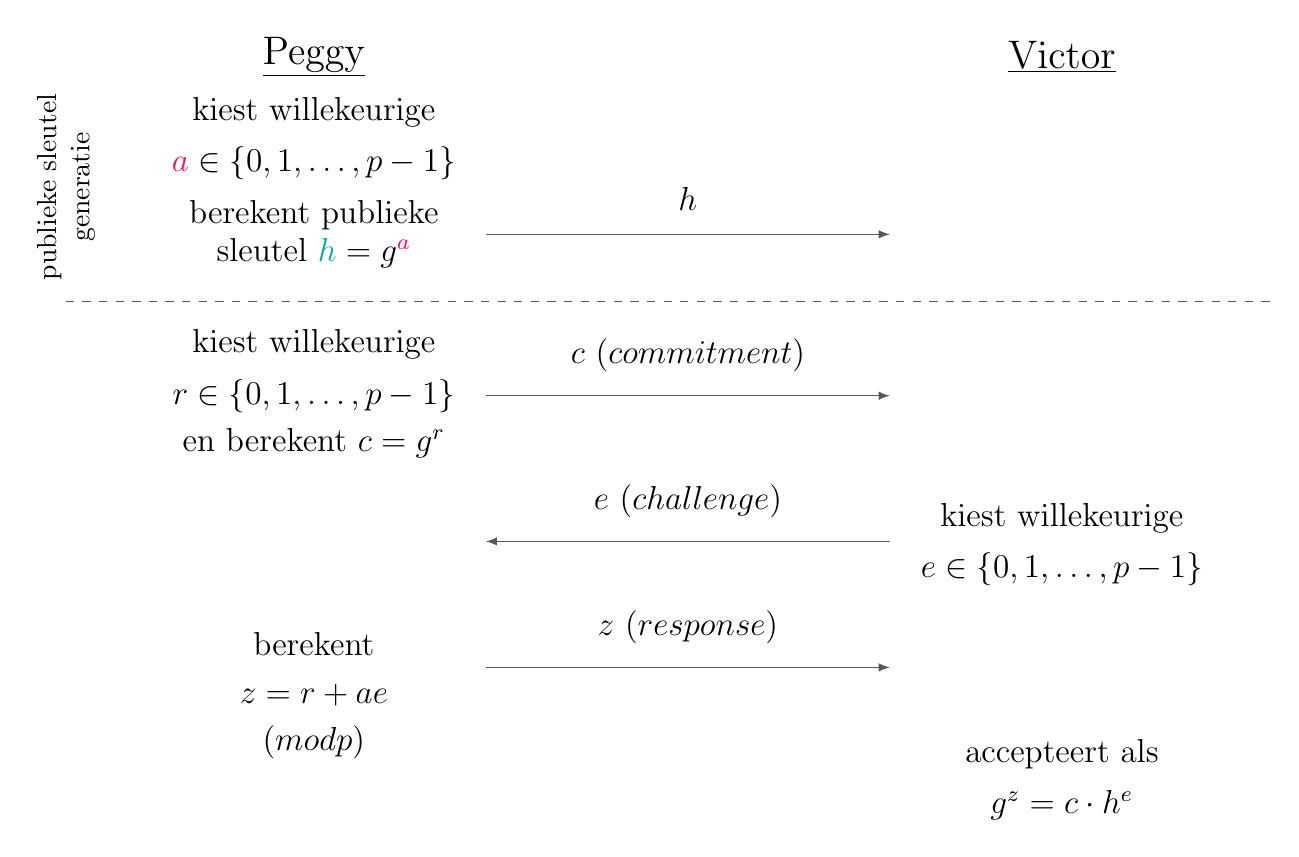
\begin{tikzpicture}[
    >=latex,
    participant/.style={
        font=\Large
    },
    textline/.style={
        font=\large,
        align=center
    },
    formula/.style={
        font=\large
    },
    message/.style={
        ->,
        thin,
        draw=black!65,
        shorten >=1pt,
        shorten <=1pt
    },
    separator/.style={
        dashed,
        thin,
        draw=black!65
    }
]

% Horizontal positions
\def\PeggyX{0}
\def\VictorX{9.5}

% ==================================================
% Participants
% ==================================================

\node[participant] at (\PeggyX,6.0)
    {\underline{Peggy}};

\node[participant] at (\VictorX,6.0)
    {\underline{Victor}};

% ==================================================
% Public-key generation
% ==================================================

\node[
    rotate=90,
    textline,
    font=\normalsize
] at (-3.15,4.35)
    {publieke sleutel\\generatie};

\node[textline] at (\PeggyX,5.30)
    {kiest willekeurige};

\node[formula] at (\PeggyX,4.65)
    {$\textcolor{WildStrawberry}{a}\in\{0,1,\ldots,p-1\}$};

\node[textline] at (\PeggyX,3.75)
    {berekent publieke\\sleutel $\textcolor{Emerald}{h}=g^{\textcolor{WildStrawberry}{a}}$};

% Peggy sends h to Victor
\draw[message]
    (2.15,3.75)
    --
    node[above=5pt, formula] {$h$}
    (7.35,3.75);

% ==================================================
% Separator
% ==================================================

\draw[separator]
    (-3.15,2.90) -- (12.15,2.90);

% ==================================================
% Commitment
% ==================================================

\node[textline] at (\PeggyX,2.35)
    {kiest willekeurige};

\node[formula] at (\PeggyX,1.70)
    {$r\in\{0,1,\ldots,p-1\}$};

\node[textline] at (\PeggyX,1.10)
    {en berekent $c=g^r$};

% Peggy sends commitment c
\draw[message]
    (2.15,1.70)
    --
    node[above=5pt, formula]
    {$c\ \text{(commitment)}$}
    (7.35,1.70);

% ==================================================
% Challenge
% ==================================================

\node[textline] at (\VictorX,0.15)
    {kiest willekeurige};

\node[formula] at (\VictorX,-0.50)
    {$e\in\{0,1,\ldots,p-1\}$};

% Victor sends challenge e to Peggy
\draw[message]
    (7.35,-0.15)
    --
    node[above=5pt, formula]
    {$e\ \text{(challenge)}$}
    (2.15,-0.15);

% ==================================================
% Response
% ==================================================

\node[textline] at (\PeggyX,-1.45)
    {berekent};

\node[formula] at (\PeggyX,-2.10)
    {$z=r+ae$};

\node[formula] at (\PeggyX,-2.70)
    {$(\operatorname{mod} p)$};

% Peggy sends response z
\draw[message]
    (2.15,-1.75)
    --
    node[above=5pt, formula]
    {$z\ \text{(response)}$}
    (7.35,-1.75);

% ==================================================
% Verification
% ==================================================

\node[textline] at (\VictorX,-2.85)
    {accepteert als};

\node[formula] at (\VictorX,-3.50)
    {$g^z=c\cdot h^e$};

\end{tikzpicture}